\documentclass[11pt]{article}

\usepackage{fullpage}
\usepackage{graphicx}
\usepackage[utf8]{inputenc}
\usepackage{setspace}
\doublespacing

\title{Heterogeneous Network Simulator Design Review}
\author{Matthew Leeds\\
	Tyler Allen\\}
\date{\today}

\begin{document}
\maketitle

{\setlength{\parindent}{0cm} \large \textbf{Abstract}}

While the Internet was originally designed for computers with stable connections 
that rarely changed location, the number of mobile devices online has grown 
rapidly in recent years. Additionally, the landscape of wireless access 
technologies has become more diverse, with WiFi, 3G/4G cellular networks, and 
WiMax often overlapping geographically. In this environment, devices often have 
multiple Internet connection options, but not enough information to know which 
connection would maximize throughput for them or for all devices competing for 
bandwidth. In theory, a Global Resource Controller (GRC) which has knowledge 
of all devices' bandwidth demands and connection options could allocate devices 
to networks in an optimal way. We seek to create a simulation of just such an 
environment in order to further understanding of these systems, and potentially 
for use as an educational tool. This paper will give an overview of the theory 
behind our project, and detail on the implementation that has been completed 
thusfar.

\section{Overview}
\subsection{Modern Wireless Connectivity}
~\indent Modern Wireless Devices are self-serving. A smart phone can be connected to a
4G network, a 3G network, an LTE network, a Wi-Max network, a WiFi network, 
or any other type of network for which the device contains an appropriate 
radio receiver. The device itself connects to the network chosen by the user. 
This is generally an easy choice for the user; if the 4G network has a 
low signal strength, it is easy to switch to a local wireless network when one 
is available. This seems effective from the perspective of the device owner, 
but having every wireless device owner select their own network of preference 
may not be an optimal setup.

\subsection{A Proprosal}
~\indent A better approach may be to have a device controlling the network distribution
in a local area. A device called a Global Resource Controller (GRC) could receive
data about devices and network traffic and make a decision about which network
each individual device should use. This requires what we will call a Heterogenous 
Network (HetNet). HetNets are a composition of all the available wireless 
networks in an area; in our model, a device could make a seamless transition
between these networks at the behest of the GRC. The GRC's job is to ensure 
that the devices in a HetNet are allocated to networks in an optimal manner.
Optimality could depend on a number of variables; our goal could be to maximize
bandwidth, cost efficiency, or a number of other variables. Our goal is 
to design a tool that can simulate this kind of environment to allow students 
a more visual experience when learning this concept, as well as allowing research
to be done into the feasibility of this kind of setup.

\subsection{Our Tool}
~\indent We are in the process of designing a web tool that allows a user to design a 
visual model of a HetNet. We believe that these types of optimality problems
can be represented as Linear Programs and then solved. Our HetNet simulation
should be capable of taking a given HetNet, optimizing it, and returning the 
results in a visual fashion. In the next section, we will discuss the 
design and implementation of this tool.


\section{Software Design}

\begin{center}
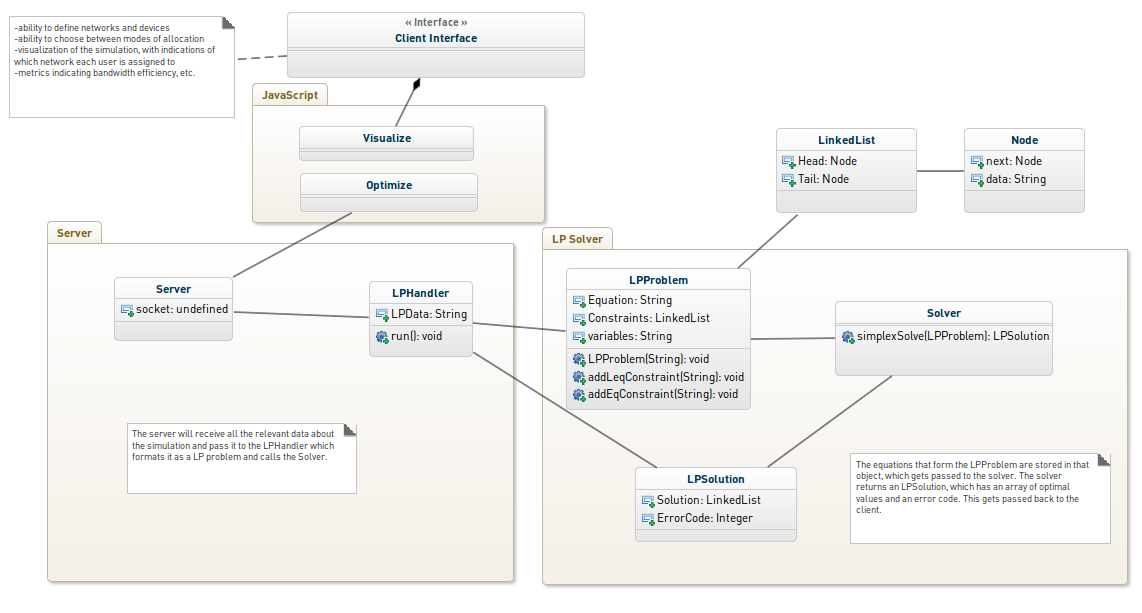
\includegraphics[width=600px, angle=270]{model.png}
\end{center}

\subsection{Overview}
~\indent As seen above, our web tool uses a typical web client-server model. The web client
will expose a GUI to the user, allowing them to build a visual model of a 
HetNet. Once the user is satisfied with their model, it will be submitted to the 
server. The server will request a solution to a Linear Program using the information 
from the HetNet model. This Linear Program will then be submitted to our Linear
Program Solver. If all goes well, a solution will be generated and returned to 
the client in some visual fashion. We are in the process of creating an 
error handling system in the event that problems generated are infeasible or 
degenerate. 

\subsection{Implementation}
~\indent The client will be created using JavaScript libraries for creating the visual 
elements and a JSON message passing system for communication to the server.
The server will be running a PHP backend which will invoke optimized
C++ code containing the Solver logic. The logic is an implementation of the two-phase
simplex method. We have used the tool \textit{SWIG}~\cite{swig} to generate  
PHP to C++ bindings. 

\subsection{Solver Design}
~\indent The Simplex Solver has been designed in a typical object oriented fashion. 
It specifies a format for Linear Programs which is exposed by the Linear Program
class. Linear Programs can be created and constraints can be added before 
the Linear Program is passed to the Solver. The Solver is an implementation of 
the Singleton design pattern, allowing for a single, lightweight, lazily generated 
object to handle any number of threaded accesses. This is with the intention of 
adding support for "dynamic models"; models that will track devices in the HetNet
over a specific timeframe; this could only be done in a timely manner using 
multiple threads to generate the response. 

\section{Details on the Linear Programming Solver}

~\indent Our Linear Programming solver uses the Two Phase 
Simplex Method to solve any feasible, bounded optimization problem in standard form.
    \subsection{Input}
~\indent Our solver handles problems in the form:~\cite{chvatal83}
\begin{eqnarray*}
\mbox{maximize}& \sum\limits_{j=1}^n c_jx_j\\
\mbox{subject to}& \sum\limits_{j=1}^n a_{ij}x_j \leq b_i\mbox{\ \ }(i \in I)\\
& \sum\limits_{j=1}^n a_{ij}x_j = b_i\mbox{\ \ }(i \in E)
\end{eqnarray*}

~\indent Since minimization problems can be written as maximizations by negating each variable, and similarly $\geq$ constraints can be negated to become $\leq$ ones, our solver only accepts three types of data:
\begin{enumerate}
\item precisely one objective equation with one or more decision variables (in its maximization form)
\item zero or more inequality constraints (in the $\leq$ form)
\item zero or more equality constraints
\end{enumerate}
...given that there is at least one constraint of some kind (otherwise the problem is unbounded).\\

\subsection{Algorithm}
\textbf{Phase I}\\
~\indent If $$E = \emptyset  \land  \forall i \in I, b_i \geq 0$$ Phase I is skipped and the standard Simplex algorithm is applied.~\cite{wolfram} Otherwise, an auxiliary problem is formed to test the feasibility of the original problem. Namely,~\cite{wolfram}
\begin{eqnarray*}
\mbox{maximize}& \sum\limits_{i=1}^m (-x_{n+i})\\
\mbox{subject to}& \sum\limits_{j=1}^n a_{ij}x_j + w_ix_{n+i} \leq b_i\mbox{\ \ }(i \in I)\\
 & \sum\limits_{j=1}^n a_{ij}x_j + w_ix_{n+i} = b_i\mbox{\ \ }(i \in E)\\
 & \sum\limits_{j=1}^n a_{ij}x_j - w_ix_{n+i} = b_i\mbox{\ \ }(i \in E)\\
 & x_{n+i} \geq 0\mbox{\ \ }(i = 1, 2,...,m)
\end{eqnarray*}
given that $w_i = 1$ whenever $b_i \geq 0$ and $w_i = -1$ whenever $b_i < 0$~\cite{chvatal83} and with $m$ being the number of constraint equations and $n$ being the number of decision variables. Once this table is formed, the following steps are performed.
\begin{enumerate}
\item For all equations where $b_i < 0$, multiply the row by -1.~\cite{wolfram}
\item For every column, sum all rows except the objective equation and subtract this value from the objective equation coefficient in that column.~\cite{wolfram}
\item Calculate an upper bound on the number of iterations, specifically $e \choose l$~\cite{chvatal83}, where $e$ is the number of candidates for entering the basis (the number of columns) and $l$ is the number of candidates for leaving it (the number of rows). 
\item Loop through the following code until we've either solved the problem (all objective equation coefficients are nonnegative) or exceeded the aforementioned maximum iterations.
  \begin{enumerate}
  \item Choose the column with the most negative objective equation coefficient as the pivot column.~\cite{wolfram}
  \item Choose the row in that column with the smallest positive $\frac{b_i}{a_{ij}}$ as the pivot row.~\cite{wolfram}
  \item Pivot on that column and row by dividing every entry in the pivot row by the value at the intersection of the pivot row and column, and then multiplying every other row by a suitable multiple of the pivot row such that their value in the pivot column becomes zero.~\cite{chvatal83}
  \end{enumerate}
\item If the related problem's optimal value is 0, the original problem is solvable and the optimal solution to the auxilary problem provides a Basic Feasible Solution for the original.~\cite{chvatal83} Transfer the first $m$ rows and $n+m$ columns of the auxilary problem's table to the original table, as well as the objective equation's row.
\end{enumerate}

\noindent \textbf{Phase II}\\
Given that Phase I indicated the problem is solvable, start from the Basic Feasible Solution (BFS) given by Phase I and implement the standard simplex method to optimize it, looping through the following steps:
\begin{enumerate}
\item If the table was produced by Phase I, choose the minimum objective equation coefficient as the pivot column.~\cite{chvatal83} Otherwise if Phase I was skipped, choose the maximum.~\cite{wolfram} A nonnegative minimum in the former case~\cite{chvatal83} or a nonpositive maximum in the latter~\cite{wolfram} indicate a solved problem.
\item If all entries in the pivot column are $\leq 0$, the problem is unbounded.~\cite{chvatal83} Otherwise, the row in that column with the smallest positive $\frac{b_i}{a_{ij}}$ is the pivot row.~\cite{chvatal83}
\end{enumerate}
If a solution was found, all decision variables are assumed to have the value 0 unless their column $i$ contains exactly one 1 and the rest 0's, in which case that row's $b_i$ value is the value of that decision variable in the optimal solution.~\cite{chvatal83} These values and the optimal value of the objective equation are returned to the caller.

\section{Questions}

\begin{itemize}
\item Is it necessary to duplicate each equality constraint in Phase I with opposite values for the artificial variables, $w_{n+i}$? Would we have to change anything else in our process if we removed that step?
\item Is it safe to delete all artificial variable columns at the end of Phase I, regardless of if they're in the basis at that point, or do they have to be pivoted out of the basis to maintain feasibility and consistency with the original problem?
\end{itemize}

\section{Future Work}

~\indent In the near-term future, we are going to implement a web interface for the heterogeneous network simulator, which will allow the user to specify parameters and visualize the system's allocations. Longer-term, the project may be extended to a larger problem domain. For example, more allocation algorithms could be added.

\begin{thebibliography}{9}
\bibitem{swig}
  SWIG 3.0,
  William Fulton, et al.  
  GNU GPL v3.
  http://swig.org/.
    
\bibitem{chvatal83}
  Vašek Chvátal,
  Linear Programming.
  W. H. Freeman and Company, New York,
  1983.
  
\bibitem{wolfram}
  "Two-Phase Simplex Method" from the Wolfram Demonstrations Project.\\
  http://demonstrations.wolfram.com/TwoPhaseSimplexMethod/.

\end{thebibliography}  
       
\end{document}
